%%%%%%%%%%%%%%%%%%%%%%%%%%%%%%%%%%%%%%%%%%
% Engineering problems / LaTeX Template
%		Semester 6
%		Institut d'Optique Graduate School
%%%%%%%%%%%%%%%%%%%%%%%%%%%%%%%%%%%%%%%%%%
%	6N-IntNum-BlocVI
%%%%%%%%%%%%%%%%%%%%%%%%%%%%%%%%%%%%%%%%%%
%
% Created by:
%	Julien VILLEMEJANE - 16/sept/2026
%	
%
%%%%%%%%%%%%%%%%%%%%%%%%%%%%%%%%%%%%%%%%%%
% Professional Newsletter Template
% LaTeX Template
% Version 1.0 (09/03/14)
%
% Created by:
% Bob Kerstetter (https://www.tug.org/texshowcase/) and extensively modified by:
% Vel (vel@latextemplates.com)
% 
% This template has been downloaded from:
% http://www.LaTeXTemplates.com
%
% License:
% CC BY-NC-SA 3.0 (http://creativecommons.org/licenses/by-nc-sa/3.0/)
%
%%%%%%%%%%%%%%%%%%%%%%%%%%%%%%%%%%%%%%%%%

\documentclass[a4paper,11pt,titlepage]{article} % The default font size is 10pt; 11pt and 12pt are alternatives

%%%%%%%%%%%%%%%%%%%%%%%%%%%%%%%%%%%%%%%%%%%%%%%%%%%%%%%%%%%%%%%%%%%%%%%%%%%%%%%%%%%%%%%%%%%%%%%%%%%%%%%%%%%%%%%%%%%%%%%%%%%%%%%%%%%%%%%%%%%%%%%%%%%%%%%%%%%%%%%%%%%%%%%%%%%%%%%%%%%%%%%%%%%%%%%%%%%%%%%%%%%%%%%%%%%%%%%%%%%%%%%%%%%%%%%%%%%%%%%%%%%%%%%%%%%%
\usepackage{./opto_elec_villemejane}

%%%%%%%%%%%%%%%%%%%%%%%%%%%%%%%%%%%%%%%%%%%%%%%%
%%%%%%%%%%%%%%%%%%%%%%%%%%%%%%%%%%%%%%%%%%%%%%%%
\begin{document}


% Page de garde
\begin{titlepage}

\begin{center}
	\begin{minipage}{2.5cm}
	\begin{center}
		
\includegraphics[width=8cm]{./images/Logo-LEnsE.png}
	\end{center}
\end{minipage}\hfill
\begin{minipage}{10cm}
	\begin{center}
	\textbf{Institut d'Optique Graduate School }\\[0.1cm]
    \textbf{\textsc{\Large Interfaçage Numérique}}


	\end{center}
\end{minipage}\hfill


\vspace{1.5cm}


{\large \bfseries Travaux Pratiques} \\[0.2cm]
Semestre 6

\vspace{1.5cm}
% Title
\rule{\linewidth}{0.3mm} \\[0.4cm]
{ \huge \bfseries\color{violet_iogs} Vision Industrielle \\[0.4cm] }
\rule{\linewidth}{0.3mm} \\[0.2cm]
{ \large \bfseries\color{violet_iogs} 2 séances\\
Détection d'objets : formes et couleurs}
\rule{\linewidth}{0.3mm} \\[1cm]


\bigskip

\begin{center}
	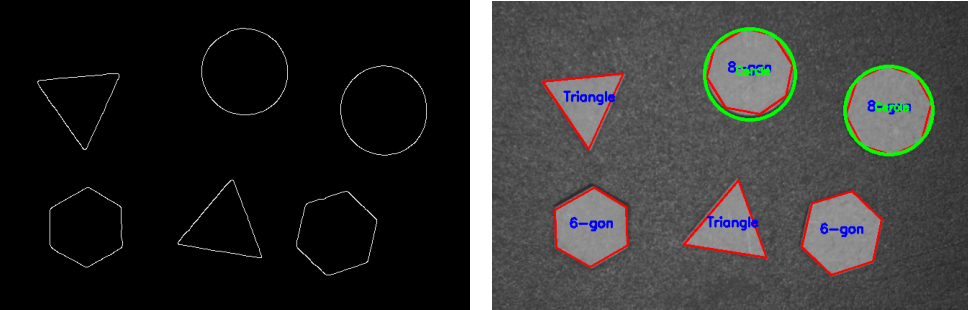
\includegraphics[width=0.9\textwidth]{./images/vi_shapes_intro.png}
\end{center}

\vfill

\textit{Ce sujet est disponible au format électronique sur le site du LEnsE - https://lense.institutoptique.fr/ dans la rubrique Année / Première Année / Interfaçage Numérique S6 / Bloc 2 Vision Industrielle.}

\vspace{1.5cm}

\begin{minipage}{5cm}
\begin{center}

\includegraphics[width=3cm]{./images/logocc}\\
\small
  © 2025 by LEnsE-IOGS 
\end{center}
\end{minipage}

% Bottom of the page
%{\textbf{\large {Année universitaire} 2024-2025}}

\end{center}
\end{titlepage}

\newpage
\strut % empty page


\textit{Ce sujet a été co-conçu par une équipe d'étudiant$\cdot$es - Joséphine BECHU, Justine GABRIEL et Paul CHENEAU - lors d'un projet DEPhI de 2A - 2025-2026 - et l'équipe pédagogique d'Interfaçage Numérique.}



\newpage
\strut % empty page

%%%%%%%%%%%%%%%%%%%%%%%%%%%%%%%%%%%%%%%%%%%%%%%%
%%%%%%%%%%%%%    A A V

\section{Vision Industrielle}


La \textbf{vision industrielle} est une technologie qui permet à des machines d'\textbf{analyser automatiquement des scènes} pour \textbf{contrôler}, \textbf{guider} ou \textbf{inspecter} des objets sur des processus de production. Elle repose sur l'utilisation de \textbf{caméras}, d'\textbf{optique}, d'\textbf{éclairages} spécifiques (ou contraints), de \textbf{capteurs} et d'algorithmes de \textbf{traitement d'image}. 

\begin{center}
	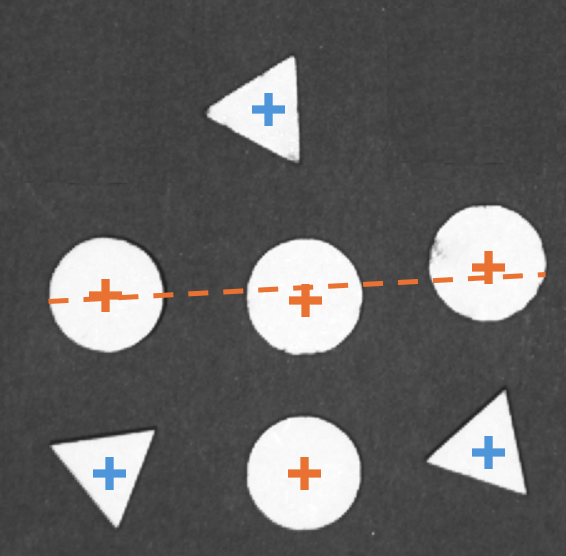
\includegraphics[width=0.3\textwidth]{./images/forms_toe.png} \quad
	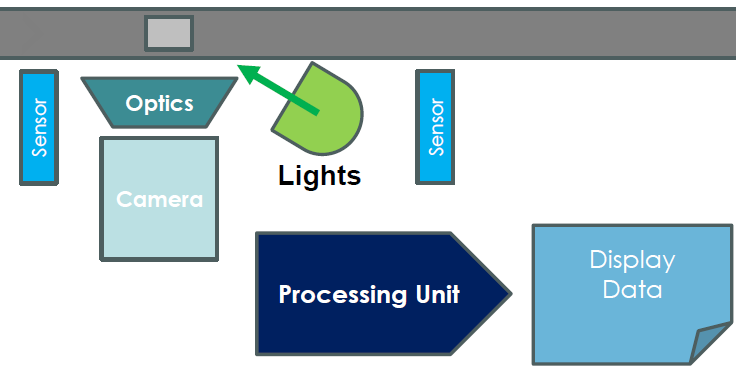
\includegraphics[width=0.5\textwidth]{./images/vi_chaine.png}
\end{center}

Elle a pour but de \textbf{prendre des décisions automatiques} (ou aider l'être humain dans sa prise de décision) vis-à-vis d'un (ou plusieurs) objet(s) dans une scène spécifique : détecter des défauts ou des irrégularités, compter ou trier..., en rejetant ou validant automatiquement des produits, tout en assurant une constance de la qualité et de la répétabilité des opérations. 

\medskip

\section{Au semestre 5...}

A travers un TP, vous avez pris en main un \textbf{banc de Vision industrielle}, incluant : une caméra, un objectif, un éclairage et une interface de pilotage. Vous avez pu \textbf{observer l'impact} de l'ensemble de ces éléments \textbf{sur l'image finale} : temps d'intégration, uniformité de l'éclairage, contraste entre les objets...

\medskip

Dans un second TP, vous avez pu \textbf{appréhender les premières briques de traitement d'image} (via la bibliothèque OpenCV) : données d'une image numérique, histogramme, flou dans une image, opérations d'ouverture/fermeture... Ces étapes sont essentielles pour \textbf{préparer l'image à la segmentation et la classification} des objets qu'elle contient.

\medskip

\section{Dans ces deux nouvelles séances...}

Lors de ce semestre, en deux séances, vous allez \textbf{mettre en place deux systèmes indépendants d'inspection de pièces}, en "temps réel" sous caméra, pour se rapprocher des systèmes industriels :

\medskip

\begin{itemize}
	\item le premier permettant de \textbf{détecter la couleur d'un objet} placé sous la caméra (cubes)
	\item le second permettant de \textbf{détecter l'alignement de formes sur une grille}, en se basant sur la règle du jeu du Morpion (ou \textit{Tic Tac Toe} en anglais).
\end{itemize}

\newpage
\section{Acquis d'Apprentissages Visés (AAV)}
%%%%%%%%%%%%%%%%%%%%%%%%%%%%%%%%%%%%%%%%%%%%%%%%
%%%%%%%%%%%%%    A A V

À la fin des 2 séances autour de la \textbf{Vision Industrielle}, les étudiant$\cdot$es seront capable de :

\begin{itemize}
	\item Réaliser un prototype d'inspection ou de mesure simple (tri d'objets)
\end{itemize}

\medskip

%%%%%%%%%%%%%%%%%%%%%%%%%%%%%%%%%%%%%%%%%%%%%%%%
%%%%%%%%%%%%%    Ressources

\section{Ressources}

Un \textbf{fichier archivé}, nommé \_STEP\_BY\_STEP\_S6.ZIP, regroupant l'ensemble des codes à tester au cours de la séance de découverte d'OpenCV, ainsi que les images à traiter, est à téléchargé sur le site du LEnsE : 

\textbf{Année / Première Année / Interfaçage Numérique S6 / Bloc 2 – Vision Industrielle / Ressources}

\vspace{0.5cm}

\begin{itemize}
	\item Téléchargez ce fichier dans un répertoire du disque dur \fbox{\textbf{U:}} de l'ordinateur.
	\item Faites un clic droit sur le fichier \textit{zip} puis \textbf{Extraire tout}. Décompressez l'archive.
\end{itemize}



\section{Accumulation de preuves / Méthode de travail}

Il est conseillé pour ces TP de \textbf{créer un nouveau projet PyCharm} sur votre session (\textit{attention à l'endroit où vous stockerez ce projet - U: sur les sessions Windows de l'IOGS}).

Les différents algorithmes que vous serez amenés à modifier ou créer, pourront vous resservir dans d'autres projets. Nous vous conseillons donc fortement de les \textbf{sauvegarder} précieusement et de les \textbf{commenter} autant que possible afin de retrouver rapidement les principes mis en jeu derrière les fonctionnalités de OpenCV.

\medskip

Il serait également pertinent de votre part de rédiger un \textbf{journal de bord} sur cette série de TP en incluant les résultats (images, histogrammes...) et vos analyses des fonctionnalités et de leur intérêt en traitement d'images.



\subsection{Validation de la compétence C4 / Valider une solution technologique}

Il est également crucial pour les chaînes de production, par exemple, d'assurer une \textbf{cadence de fabrication et de validation importante}. Les algorithmes de détection doivent donc pouvoir s'exécuter rapidement et la vitesse de défilement des pièces sous le système imageant peut devenir limitant.

Il est enfin nécessaire de valider ces systèmes de prise de décision en mesurant leur \textbf{taux d'erreur} vis-à-vis des grandeurs à tester. Ce taux d'erreur doit être proche de 0, une tolérance peut être acceptée et peut être différente selon le type de défauts à identifier, le type de matériaux utilisés...

\medskip

Dans le cadre de ces TP, il sera important de \textbf{définir des protocoles de test pour ces deux aspects} (temps d'exécution des algorithmes et taux d'erreur) et de donner quelques mesures quantitatives.

\newpage
\pagestyle{empty}


%%%%%%%%%%%%%%%%%%%%%%%%%%%%%%%%%%%%%%%%%%%%%%%%
%%%%%%%%%%%%%    A A V / Objectifs

\section{Objectif des deux séances}

\textit{L'utilisation d'un banc de vision industrielle est indispensable pour les deux séances.}

\subsection{TP1 - Manipulations avancées sous OpenCV / Formes et couleurs}

Dans cette première séance, vous allez devoir mettre en place un système de détection d'objets (formes simples) et de couleurs, afin d'identifier la couleur du (ou des) cube(s) de couleur que vous mettrez sous la caméra.

\medskip

Des \textbf{scripts} vont vous permettre, \textbf{pas à pas}, de :

\begin{itemize}
	\item récupérer le flux de la caméra depuis un OpenCV (calibration de la caméra, boucle d'acquisition des images...)
	\item détecter des formes (à partir de la quantité de contours - segments - d'un objet)
	\item détecter la couleur de ces objets (utilisation d'espaces colorimétriques appropriés)
\end{itemize}

\medskip

Vous devrez, à partir de ces scripts de base, \textbf{réaliser} et \textbf{faire valider une application simple} mais \textbf{robuste} de détection de la couleur d'objets placés sous la caméra.

\subsection{TP2 - Détection d'objets - Contrôle qualité}

L'objectif final de ce second TP est de \textbf{détecter le nombre d'objets d'une forme particulière et leur alignement sur une grille}, en temps réel sous caméra.

On se basera sur la règle du \textbf{jeu du Morpion} (ou \textit{Tic Tac Toe} en anglais) qui oppose deux joueurs qui doivent aligner 3 marques (de même forme ou couleur) sur une grille de 3 x 3 cases. 

\bigskip

Premiers essais sur une grille de jeu TicTacToe (morpion) :

\begin{center}
	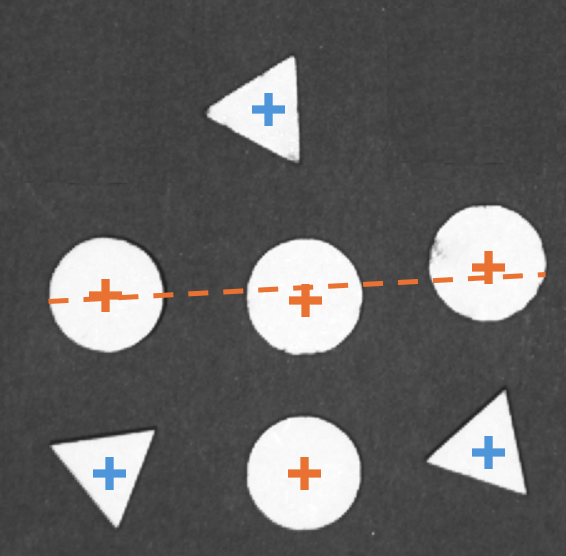
\includegraphics[width=0.3\textwidth]{./images/forms_toe.png}
\end{center}

Cette mission "ludique" est cependant très proche des \textbf{tâches d'inspection en industrie}, afin par exemple de valider si les pièces requises pour un assemblage sont bien présentes (simuler le packaging d'un produit fini - 6 pièces de forme et de couleurs distinctes par exemple).

On pourra ajouter également des mesures de surface des pièces, de colorimétrie pour valider la couleur des dépôts faits sur les pièces... pour vérifier leur \textbf{conformité à un cahier des charges}.

\medskip



%%%%%%%%%%%%%%%%%%%%%%%%%%%%%%%%%%%%%%%%%%%%%%%%
%%%%%%%%%%%%%%%%%%%%%%%%%%%%%%%%%%%%%%%%%%%%%%%%
%%  TP 1




\newpage
\begin{center}
	\begin{minipage}{2.5cm}
	\begin{center}
		
\includegraphics[width=5cm]{./images/Logo-LEnsE.png}
	\end{center}
\end{minipage}\hfill
\begin{minipage}{10cm}
	\begin{center}
	\textbf{Institut d'Optique Graduate School }\\[0.1cm]
    \textbf{Interfaçage Numérique}


	\end{center}
\end{minipage}\hfill


\vspace{2cm}


{\Large \bfseries \textsc{Interfaçage Numérique}} \\[0.5cm]
{\large \bfseries Travaux Pratiques} \\[0.2cm]
Semestre 6

\vspace{1cm}

% Title
\rule{\linewidth}{0.4mm} \\[0.4cm]
{ \Large \bfseries\color{violet_iogs} TP1 - Manipulations avancées sous OpenCV \\ Formes et couleurs \\[0.4cm] }
\rule{\linewidth}{0.4mm} \\[1cm]

\end{center}

\vfill


\bigskip

\section{Méthode de travail (conseillée)}


Une partie des algorithmes de traitement sont donnés. Il est fortement conseillé de \textbf{réaliser une analyse poussée} de chacune des étapes de ces algorithmes afin de comprendre l'intérêt de l'utilisation de ces techniques de base.

\medskip

Vous pouvez par exemple \textbf{décrire ces algorithmes} par l'intermédiaire d'un graphique (algorigramme) et \textbf{afficher les résultats intermédiaires} (et en faire une capture d'écran) tout en \textbf{commentant les résultats}. 

\medskip

\textbf{Faites des copies des scripts fournis}, afin de garder une trace des évolutions que vous avez apportés.



\newpage

%%%%%%%%%%%%%%%%%%%%%%%%%%%%%%%%%%%%%%%
%%%%%%%%%%%% FLUX Camera
\section{A - Flux de la caméra {[30 min]}}

\Manip Allumer l'\textbf{éclairage annulaire} du banc (trois couleurs). Placer un \textbf{fond uniforme} sous l'éclairage (feuille blanche, paillasse, fond sombre...) et quelques objets (cubes de couleur par exemple).

\Manip Ouvrir le fichier \textsc{101\_flux\_camera\_lensepy\_simple.py} du répertoire des codes à tester.

\Manip Exécuter ce code.

\textit{Si la caméra est bien connectée en USB à l'ordinateur, vous devriez voir s'afficher son flux. Ce script se base sur la bibliothèque \textbf{lensepy\_app} développée par le LEnsE.}

\Quest Détaillez les parties du script fourni. 

\Quest De quelle taille est l'image ?

\noindent \rule{\linewidth}{1pt}

\Manip Ouvrir le fichier \textsc{102\_flux\_camera\_lensepy\_histo.py} du répertoire des codes à tester. Exécuter ce code. Modifier le temps d'exposition pour obtenir une image exploitable.

\Quest Sur quel(s) critère(s) vous basez-vous pour valider l'exploitabilité de votre prise d'image ?

\noindent \rule{\linewidth}{1pt}

\Manip Ouvrir le fichier \textsc{103\_flux\_camera\_lensepy\_process.py} du répertoire des codes à tester. Exécuter ce code.

\Quest Détaillez les parties du script fourni.


%%%%%%%%%%%%%%%%%%%%%%%%%%%%%%%%%%%%%%%
%%%%%%%%%%%% FORMES
\section{B - Détection de formes {[60 min]}}

\Manip Ouvrir le fichier \textsc{111\_detection\_forme.py} du répertoire des codes à tester. Exécuter ce code.

\Quest Détaillez les parties du script fourni.

\Quest Ce code fournit-il un résultat satisfaisant ? A quoi servent notamment les paramètres \textsc{MIN\_AREA} et \textsc{APPROX\_FACTOR} ?

\Quest Et dans le cas de la seconde image proposée (\textsc{formes\_blanc\_30ms.png}), le résultat est-il satisfaisant ? Quel est la différence majeure entre ces deux images ?

\noindent \rule{\linewidth}{1pt}

\Manip Ouvrir le fichier \textsc{112\_detection\_forme\_plus.py} du répertoire des codes à tester. Exécuter ce code.

\Quest Quelle étape a été ajoutée par rapport à la version précédente ? Le résultat est-il satisfaisant ?

\noindent \rule{\linewidth}{1pt}

\Manip Ouvrir le fichier \textsc{113\_detection\_forme\_cercles.py} du répertoire des codes à tester. Exécuter ce code.

\Quest Détaillez les étapes de ce code et le résultat obtenu.

\Quest Dans le cas de la seconde image proposée (\textsc{formes\_blanc\_30ms.png}), le résultat est-il satisfaisant ? 

\Manip Ouvrir le fichier \textsc{113b\_detection\_forme\_cercles\_plus.py} du répertoire des codes à tester. Exécuter ce code.

\Quest Quelle étape a été ajoutée par rapport à la version précédente ? Le résultat est-il satisfaisant ?

\newpage
%%%%%%%%%%%%%%%%%%%%%%%%%%%%%%%%%%%%%%%
%%%%%%%%%%%% FORMES sous flux
\section{C - Détection de formes et de couleurs sous caméra {[60 min]}}

\Manip Ouvrir le fichier \textsc{121\_flux\_camera\_crop.py} du répertoire des codes à tester. Exécuter ce code.

\Quest Que permet-il de faire ?

\noindent \rule{\linewidth}{1pt}

\Manip Ouvrir le fichier \textsc{122\_flux\_camera\_mask.py} du répertoire des codes à tester. Exécuter ce code.

\Quest Que permet-il de faire ?

\noindent \rule{\linewidth}{1pt}

\Manip A partir des scripts précédents (également ceux étudiés en section A) et des différentes observations effectuées dans la section B, mettre en place un script qui, à partir du flux de la caméra :

\begin{enumerate}
	\item Affiche le flux de la caméra 
	\item Détecte un objet de forme carrée dans l'image (cube placé sous la caméra)
	\item Affiche les valeurs RVB moyennes de l'objet
\end{enumerate}

\bigskip

\textit{Penser à régler correctement le temps d'intégration.}

\medskip

\Quest Est-il facile de déterminer la couleur d'un objet par cette méthode ?

\medskip

%%%%%%%%%%%%%%%%%%%%%%%%%%%%%%%%%%%%%%%
%%%%%%%%%%%% COULEURS
\section{D - Détection de couleurs efficace {[30 min]}}

\subsubsection{Utiliser l'espace colorimétrique HSV}

L'espace colorimétrique \textbf{HSV} (\textit{Hue, Saturation, Value}) représente les couleurs de manière intuitive en les séparant selon :

\begin{itemize}
	\item la \textbf{teinte} (Hue), qui correspond au type de couleur et est généralement exprimée comme un angle sur un cercle (rouge, vert, bleu, etc.), 
	\item la \textbf{saturation} (Saturation), qui mesure la pureté ou l'intensité de la couleur (d'une couleur vive à un gris),
	\item la \textbf{valeur} (Value), qui représente la luminosité globale.
\end{itemize} 

\medskip

Contrairement à l'espace RVB, HSV est conçu pour se rapprocher de la perception humaine, ce qui le rend particulièrement adapté aux tâches de vision par ordinateur, notamment la détection et la segmentation de couleurs, car il permet de dissocier plus facilement l'information de couleur des variations d'éclairage.

\noindent \rule{\linewidth}{1pt}

\Manip Ouvrir le fichier \textsc{131\_couleur\_hsv.py} du répertoire des codes à tester.

\Manip Exécuter ce code.

\Quest Que représentent les deux lignes de figure affichées par ce programme ?

\Quest Comment pouvez-vous interpréter les deux histogrammes ?

\noindent \rule{\linewidth}{1pt}

\Manip Ajouter un filtrage de type \textit{blur} gaussien (\textit{cv2.GaussianBlur}) sur l'image RVB \textsc{formes\_bruit.png} (noyau carré de 7x7 et $\sigma = 1.9$).

\Quest Quel est l'effet sur l'histogramme associé à cette image ? Quel serait l'inconvénient de cette technique, par rapport à la détection de couleur via l'espace HSV ?

\subsubsection{Segmenter une image en fonction de la couleur}

\Manip Ouvrir le fichier \textsc{132\_hsv\_rgb.py} du répertoire des codes à tester.

\Manip Exécuter le code.

\Quest Expliquer le principe utilisé dans chacune des segmentations, en RVB et HSV. On s'intéressera en particulier aux bornes utilisées.

\Quest Quelle méthode est la plus efficace pour détecter la couleur rouge ?

\Manip Ajouter la détection de la zone bleue, de l'image initialement ouverte, par la méthode qui vous parait la plus pertinente. Afficher une nouvelle image avec le résultat final.


\subsubsection{Segmenter une image en fonction de la couleur}

\Manip A partir du script que vous avez mis en place dans la partie C (détection d'une couleur RVB d'un objet), réaliser un script qui permet de \textbf{déterminer les valeurs HSV} des différents cubes à votre disposition.

\Manip Mesurer les valeurs HSV de chacun des cubes de couleur à votre disposition.

\Quest Quelles valeurs sont dépendantes de la quantité de photons captées par la caméra ?

\medskip

\textit{Vous pourrez également tester sur plusieurs cubes d'une même couleur pour tester la répétabilité de vos mesures et vérifier la robustesse du protocole que vous allez devoir mettre en place par la suite.}

\medskip

\textit{Cette étape servira de calibration pour la détection de la couleur des cubes que vous mettrez en place dans la section suivante.}


%%%%%%%%%%%%%%%%%%%%%%%%%%%%%%%%%%%%%%%
%%%%%%%%%%%% COULEURS
\section{E - Détection de couleurs efficace {[60 min]}}


\Manip A partir de l'ensemble des éléments précédents, vous devez mettre en place une solution technologique (script) permettant :

	\begin{enumerate}
		\item de \textbf{détecter la position d'un cube} placé sous la caméra
		\item d'\textbf{afficher la couleur du cube} (parmi les 4 possibles)
	\end{enumerate}

\textit{On ne placera dans un premier temps qu'un seul cube de couleur sous la caméra.}

\medskip	
	
\Quest Faire valider votre système ainsi que ces performances.


\noindent \rule{\linewidth}{1pt}

\Manip Etendre votre solution à plusieurs cubes placés sous la caméra.



\newpage
%%%%%%%%%%%%%%%%%%%%%%%%%%%%%%%%%%%%%%%
%%%%%%%%%%%% YUV
\section{F - Niveaux de gris {[30 min]}}

Il existe plusieurs méthodes pour transformer une image en RVB vers une image en nuance de gris.

\subsubsection{Moyenne des canaux R,V,B}

Cette méthode est la plus simple. Chaque pixel de l'image en gris est la moyenne des pixels des canaux rouge, vert et bleu de l'image en couleur :

$$Pixel_{Gray} = \frac{Pixel_{R} + Pixel_{V} + Pixel_{B}}{3}$$ 


\subsubsection{Pondération en fonction de la perception humaine}

Cette méthode est une moyenne pondérée des valeurs des pixels R, V, B de l'image couleur : 

$$Pixel_{Gray} = 0.299 \cdot Pixel_{R} + 0.587 \cdot Pixel_{V} + 0.114 \cdot Pixel_{B}$$ 


Les coefficients de cette méthode proviennent de la sensibilité relative de l'œil humain aux différentes couleurs et ont été standardisés à l'origine pour la télévision analogique (NTSC). Ils sont aujourd'hui utilisés comme une approximation fidèle de la perception visuelle de la luminosité.


\noindent \rule{\linewidth}{1pt}

\Manip Ouvrir le fichier \textsc{141\_colorspace.py} du répertoire des codes à tester.

\Quest Que fait ce programme ? 

\Manip Comparer les images obtenues par la moyenne classique et la moyenne pondérée.

\subsubsection{Utiliser l'espace colorimétrique YUV}

L'espace colorimétrique RVB est très utilisé dans le domaine du numérique (affichage, acquisition d'images) pour sa facilité de mise en oeuvre.

Cependant, ce n'est \textbf{pas} le plus \textbf{adapté vis-à-vis de la perception humaine} où la luminance et la couleur sont séparées.

Des espaces comme YUV, YIQ, ou YCbCr séparent la composante de luminance (Y) des composantes de chrominance (U et V).

\Manip Ouvrir le fichier \textsc{142\_colorspace \_yuv.py} du répertoire des codes à tester.

\Manip Comparer alors l'image en niveau de gris obtenue par la méthode de moyennage pondérée et le canal Y de cette conversion.

\Quest Que pouvez-vous conclure sur la méthode de calcul utiliser pour la luminance (Y) ?

\medskip

\noindent \rule{\linewidth}{1pt}

Il existe d'autres espaces colorimétriques dans le domaine numérique. Voici un résumé non exhaustif :

\begin{center}
\begin{tabular}{|c|c|}
\hline
\textbf{Espace colorimétrique} & \textbf{Avantages} \\ \hline
\textbf{RGB} & Simple, utilisé pour les écrans et le rendu des couleurs. \\ \hline
\textbf{HSV / HSL} & Intuitif pour manipuler la couleur (teinte, saturation). \\ \hline
\textbf{YUV / YCbCr} & Sépare luminance et chrominance. \\ \hline
\textbf{CIE-Lab} & Uniformité perceptuelle, idéal pour mesurer les différences de couleur. \\ \hline
\textbf{CMY(K)} & Optimisé pour l'impression. \\ \hline
\textbf{XYZ} & Modèle basé sur la perception humaine. \\ \hline
\end{tabular}
\end{center}




\newpage

EN RESUME

(C) = caméra

(I) = images

\bigskip


\textbf{TP2}

\begin{enumerate}
	\item Détection de mires/grilles
	\begin{enumerate}
		\item (I) repères simples (correlation)
		\item (C) sous caméra
	\end{enumerate}
	\item Mires multi-échelle
	\begin{enumerate}
		\item (I) repères simples (correlation)
		\item (C) sous caméra
	\end{enumerate}
	\item Mires améliorées (à voir !! selon temps)
	\begin{enumerate}
		\item (I) repères améliorés (correlation)
		\item (C) sous caméra
	\end{enumerate}
	\item (C) \textbf{APPLI} qui repère la grille sous la caméra et détecte le quadrillage
	\item (C) \textbf{APPLI} qui repère les formes dans chaque zone de la grille
	\item (C) \textbf{APPLI} qui valide une grille de TikTakToe
	
\end{enumerate}

\newpage
%%%%%%%%%%%%%    Etape A
\subsection{CV-A - Détecter des formes {[40 min]}}

\subsubsection{Détection de contours sur une image "propre"}

\Manip Ouvrir le fichier \textsc{20\_detection\_forme.py} du répertoire des codes à tester.

\Manip Exécuter ce code.

\Quest Que fait ce programme ? A quoi correspondent les images affichées ? A quoi correspondent les données affichées ?

\noindent \rule{\linewidth}{1pt}

\Manip Modifier le paramètre MIN\_AREA (100, 1000, 10000).

\Quest A quoi sert ce paramètre ? Quelle est son unité ? Comment la transformer en unités plus conventionnelles ?

\noindent \rule{\linewidth}{1pt}

\Manip Modifier le paramètre APPROX\_FACTOR (0.01, 0.05, 0.1).

\Quest A quoi sert ce paramètre ?

\Quest A quoi correspondent les variables \texttt{cX}, \texttt{cY}, \texttt{area} et \texttt{peri} ?


\subsubsection{Détection de contours sur une image "réelle"}

L'image précédente était "propre" (sans bruits dûs au capteur par exemple). Nous allons nous intéresser à présent à une image provenant d'une chaine d'acquisition.

\Manip A partir du code précédent, ouvrir l'image \textsc{formes\_blanc\_30ms.png} du répertoire du kit d'images.

\Quest L'algorithme est-il efficace ?

\noindent \rule{\linewidth}{1pt}

\Manip Ouvrir le fichier \textsc{21\_detection\_forme\_plus.py} du répertoire des codes à tester.

\Manip Exécuter ce code.

\Quest Quelle étape est-elle ajoutée par rapport à la version précédente du code ?

\noindent \rule{\linewidth}{1pt}

\Manip Ajouter un traitement morphologique de type \textit{opening} (ouverture) sur l'image binarisée (noyau carré de 3x3, puis 5x5).

\Manip Ajouter l'affichage de l'image ainsi traitée.

\Quest Que permet cette étape dans l'algorithme de détection ? 


\subsubsection{Détection de cercles}

\Manip Ouvrir le fichier \textsc{22\_detection\_forme\_cercles.py} du répertoire des codes à tester.

\Manip Exécuter ce code.

\Quest Quelle amélioration apporte ce programme ?

\subsubsection{Détection de cercles sur une image "réelle"}

L'\textbf{algorithme de Hough} qui permet la recherche de cercles dans une image se base sur des images en nuance de gris (et non binarisée). Il s'appuie sur des gradients d'intensité et des bords continus et doux pour détecter les transitions (contours des cercles).

Il n'est donc pas possible d'utiliser une opération morphologique d'ouverture sur l'image. 


\Manip Ouvrir le fichier \textsc{23\_detection\_forme\_blur\_cercles.py} du répertoire des codes à tester.

\Manip Exécuter ce code. Vérifier que l'algorithme n'est pas efficace.

\noindent \rule{\linewidth}{1pt}

\Manip Ajouter un filtrage de type \textit{blur} gaussien (\textit{cv2.GaussianBlur}) sur l'image grise (noyau carré de 7x7 et $\sigma = 1.9$).

\Manip Ajouter l'affichage de l'image ainsi traitée.

\Quest Que permet cette étape dans l'algorithme de détection ?

\Manip Modifier la taille du noyau (3x3, 5x5, 15x15) et de la valeur de $\sigma$ (1.9, 3, 5, 10).

\Quest Quel est l'impact du choix de ces deux paramètres ?



%%%%%%%%%%%%%    Etape B
\subsection{CV-B - Détecter des couleurs {[40 min]}}

\subsubsection{Jouer avec les canaux de couleurs}

\Manip Ouvrir et afficher l'image \textsl{couleurs\_4.png} du kit d'images fourni, au format RGB.

\Manip Créer une copie de la matrice image (fonction \textsl{copy()} de Numpy). 

\Manip Forcer à 0 tous les pixels du canal bleu de la copie de l'image et afficher la nouvelle image.


\subsubsection{Utiliser l'espace colorimétrique HSV}

L'espace colorimétrique \textbf{HSV} (\textit{Hue, Saturation, Value}) représente les couleurs de manière intuitive en les séparant selon :

\begin{itemize}
	\item la \textbf{teinte} (Hue), qui correspond au type de couleur et est généralement exprimée comme un angle sur un cercle (rouge, vert, bleu, etc.), 
	\item la \textbf{saturation} (Saturation), qui mesure la pureté ou l'intensité de la couleur (d'une couleur vive à un gris),
	\item la \textbf{valeur} (Value), qui représente la luminosité globale.
\end{itemize} 

\medskip

Contrairement à l'espace RVB, HSV est conçu pour se rapprocher de la perception humaine, ce qui le rend particulièrement adapté aux tâches de vision par ordinateur, notamment la détection et la segmentation de couleurs, car il permet de dissocier plus facilement l'information de couleur des variations d'éclairage.

\Manip Ouvrir le fichier \textsc{24\_couleur\_hsv.py} du répertoire des codes à tester.

\Manip Exécuter ce code.

\Quest Que représentent les deux lignes de figure affichées par ce programme ?

\Quest Comment pouvez-vous interpréter les deux histogrammes ?

\noindent \rule{\linewidth}{1pt}

\Manip Ajouter un filtrage de type \textit{blur} gaussien (\textit{cv2.GaussianBlur}) sur l'image rgb \textsc{formes\_bruit.png} (noyau carré de 7x7 et $\sigma = 1.9$).

\Quest Quel est l'effet sur l'histogramme associé à cette image ? Quel serait l'inconvénient de cette technique, par rapport à la détection de couleur via l'espace HSV ?

\subsubsection{Segmenter une image en fonction de la couleur}

\Manip Ouvrir le fichier \textsc{24b\_hsv\_rgb.py} du répertoire des codes à tester.

\Manip Exécuter le code.

\Quest Expliquer le principe utilisé dans chacune des segmentations, en RVB et HSV. On s'intéressera en particulier aux bornes utilisées.

\Quest Quelle méthode est la plus efficace pour détecter la couleur rouge ?

\Manip Ajouter la détection de la zone bleue, de l'image initialement ouverte, par la méthode qui vous parait la plus pertinente. Afficher une nouvelle image avec le résultat final.


%%%%%%%%%%%%%    Etape B
\subsection{CV-C - Passer de la couleur à des niveaux de gris {[40 min]}}

Il existe plusieurs méthodes pour transformer une image en RVB vers une image en nuance de gris par exemple.

\subsubsection{Moyenne des canaux R,V,B}

Cette méthode est la plus simple. Chaque pixel de l'image en gris est la moyenne des pixels des canaux rouge, vert et bleu de l'image en couleur :

$$Pixel_{Gray} = \frac{Pixel_{R} + Pixel_{V} + Pixel_{B}}{3}$$ 


\subsubsection{Pondération en fonction de la perception humaine}

Cette méthode est une moyenne pondérée des valeurs des pixels R, V, B de l'image couleur : 

$$Pixel_{Gray} = 0.299 \cdot Pixel_{R} + 0.587 \cdot Pixel_{V} + 0.114 \cdot Pixel_{B}$$ 


Les coefficients de cette méthode proviennent de la sensibilité relative de l'œil humain aux différentes couleurs et ont été standardisés à l'origine pour la télévision analogique (NTSC). Ils sont aujourd'hui utilisés comme une approximation fidèle de la perception visuelle de la luminosité.

La méthode de conversion fournie par la bibliothèque OpenCV se base sur cette pondération.

\noindent \rule{\linewidth}{1pt}


\Manip Ouvrir le fichier \textsc{30\_colorspace.py} du répertoire des codes à tester.

\Quest Que fait ce programme ? A quoi sert l'instruction \textsc{cmap='gray'} de la fonction \textit{imshow} de \textit{Matplotlib} ?

\noindent \rule{\linewidth}{1pt}

\Manip Créer une image en nuance de gris utilisant la méthode de la moyenne des trois canaux. \textit{Attention aux types des données dont vous faites la moyenne...}

\Manip Afficher l'image résultante.

\Manip Comparer les images obtenues par la moyenne classique et la moyenne pondérée.


\subsubsection{Utiliser l'espace colorimétrique YUV}

L'espace colorimétrique RVB est très utilisé dans le domaine du numérique (affichage, acquisition d'images) pour sa facilité de mise en oeuvre.

Cependant, ce n'est \textbf{pas} le plus \textbf{adapté vis-à-vis de la perception humaine} où la luminance et la couleur sont séparées.

Des espaces comme YUV, YIQ, ou YCbCr séparent la composante de luminance (Y) des composantes de chrominance (U et V).

\Manip Ouvrir le fichier \textsc{31\_colorspace \_yuv.py} du répertoire des codes à tester.

\Manip Comparer alors l'image en niveau de gris obtenue par la méthode de moyennage pondérée et le canal Y de cette conversion.

\Quest Que pouvez-vous conclure sur la méthode de calcul utiliser pour la luminance (Y) ?

\medskip

\noindent \rule{\linewidth}{1pt}

Il existe d'autres espaces colorimétriques dans le domaine numérique. Voici un résumé non exhaustif :

\begin{center}
\begin{tabular}{|c|c|}
\hline
\textbf{Espace colorimétrique} & \textbf{Avantages} \\ \hline
\textbf{RGB} & Simple, utilisé pour les écrans et le rendu des couleurs. \\ \hline
\textbf{HSV / HSL} & Intuitif pour manipuler la couleur (teinte, saturation). \\ \hline
\textbf{YUV / YCbCr} & Sépare luminance et chrominance. \\ \hline
\textbf{CIE-Lab} & Uniformité perceptuelle, idéal pour mesurer les différences de couleur. \\ \hline
\textbf{CMY(K)} & Optimisé pour l'impression. \\ \hline
\textbf{XYZ} & Modèle basé sur la perception humaine. \\ \hline
\end{tabular}
\end{center}



\newpage
%%%%%%%%%%%%%%%%%%%%%%%%%%%%%%%%%%%%%%%%%%%%%%%%
%%%%%%%%%%%%%    Etape par étape

\section{Banc VI - Calibration sur flux vidéo}

On se propose dans cette partie de tester les algorithmes de détection sur un flux vidéo, sans passer par l'interface utilisée lors d'une précédente séance.

%%%%%%%%%%%%%    Etape A
\subsection{VI-A - Tester les algorithmes sur un flux vidéo {[40 min]}}

\Manip Ouvrir le fichier \textsc{camera\_flux\_lensepy\_simple.py} du répertoire des codes à tester.

\Manip Tester le programme, en ayant au préalable connecté une caméra de type Basler. Tester en particulier l'interaction avec l'utilisateur (touches 'a', 'i', 'c', 'g').

\Quest A quoi servent les options \textsc{COLOR\_MODE}  et \textsc{DISPLAY\_RATIO} ?

\Quest Faire un algorigramme (algorithme du programme en version graphique) de ce code.

\noindent \rule{\linewidth}{1pt}

\Manip Modifier le code pour ajouter une option (par exemple la lettre 'e') : permettre l'affichage de l'image subissant une érosion avec un noyau circulaire de 7x7. Tester votre code.

%%%%%%%%%%%%%    Etape B
\subsection{VI-B - Calibrer la chaîne d'acquisition {[90 min]}}


\textit{Pour cette section, les binômes étant sur des paillasses disposant d'une caméra pourront utiliser directement les images provenant de la caméra.}

\textit{Pour les autres binômes, vous pourrez vous reposer sur les images suivantes :}

\begin{itemize}
	\item \textsc{cubes\_RGB.png} : acquisition des 4 cubes de couleur sous un éclairage blanc (\textit{ring} RGB Effi-Ring) en mode BayerRG8 ;
	\item \textsc{cubes\_R.png} : acquisition des 4 cubes de couleur sous un éclairage rouge (\textit{ring} RGB Effi-Ring) en mode Mono8 ;
	\item \textsc{cubes\_G.png} : acquisition des 4 cubes de couleur sous un éclairage vert (\textit{ring} RGB Effi-Ring) en mode Mono8 ;
	\item \textsc{cubes\_B.png} : acquisition des 4 cubes de couleur sous un éclairage bleu (\textit{ring} RGB Effi-Ring) en mode Mono8 ;
	\medskip
	\item \textsc{forms.png} : acquisition d'une dizaine de pièces en bois de formes différentes sous un éclairage blanc (\textit{ring} RGB Effi-Ring) en mode Mono8 ;
	\item \textsc{forms\_toe.png} : acquisition d'une dizaine de pièces en bois de formes différentes - alignées - sous un éclairage blanc (\textit{ring} RGB Effi-Ring) en mode Mono8 ;
\end{itemize}

\bigskip

\textit{Ces images sont disponibles sur le site du LEnsE - https://lense.institutoptique.fr/ dans la rubrique Année / Première Année / Interfaçage Numérique S6 / Bloc 2 Vision Industrielle / Cubes/Formes.}



%%%%%%%%%%%%%%%%%%%%%%%%%
\subsubsection{Détecter des cubes colorés}

On se propose ici de détecter la couleur des cubes fournis (jaune, rouge, bleu et vert) de manière un peu plus automatisée et d'extraire certaines informations de ces objets (position, aire...).

\Quest Proposer une méthode (algorithme) à mettre en place pour détecter la présence d'un élément d'une des 4 couleurs à détecter, ainsi que sa position.

\Manip A partir de l'exemple \textsc{camera\_flux\_lensepy\_simple.py} (en remplaçant si besoin l'image provenant de la caméra par l'ouverture d'une image fixe), ajouter cette fonctionnalité.

\noindent \rule{\linewidth}{1pt}

\Quest Proposer une méthode (algorithme) à mettre en place pour détecter la présence de tous les éléments d'une couleur donnée et de compter le nombre d'objets présents.

\Manip A partir de l'exemple \textsc{camera\_flux\_lensepy\_simple.py} (en remplaçant si besoin l'image provenant de la caméra par l'ouverture d'une image fixe), ajouter cette fonctionnalité.

\noindent \rule{\linewidth}{1pt}

\Manip A partir de l'exemple \textsc{camera\_flux\_lensepy\_simple.py} (en remplaçant si besoin l'image provenant de la caméra par l'ouverture d'une image fixe), créer un programme qui permette de lister les cubes des 4 couleurs et d'afficher pour chacun d'eux : les coordonnées de leur centre, leur surface, la couleur...

\noindent \rule{\linewidth}{1pt}

Il est possible d'avoir une estimation du temps d'exécution d'un code en Python par la méthode proposée ci-dessous :

\begin{lstlisting}
import time

start = time.perf_counter()
# Code to evaluate
end = time.perf_counter()

print(f"Total Time : {(end - start)*1000:.2f} ms")
\end{lstlisting}

\Manip A partir de cet exemple, mesurer le temps de traitement de détection des cubes de couleurs.

%%%%%%%%%%%%%%%%%%%%%%%%%
\subsubsection{Détecter des formes particulières}

On souhaite à présent s'intéresser aux pièces en bois de 3 formes différentes (cercle, triangle, hexagone).

A terme, nous aimerions pouvoir détecter si des formes d'un même type sont alignées sur une grille (principe du jeu Tic-tac-toe).

\begin{center}
	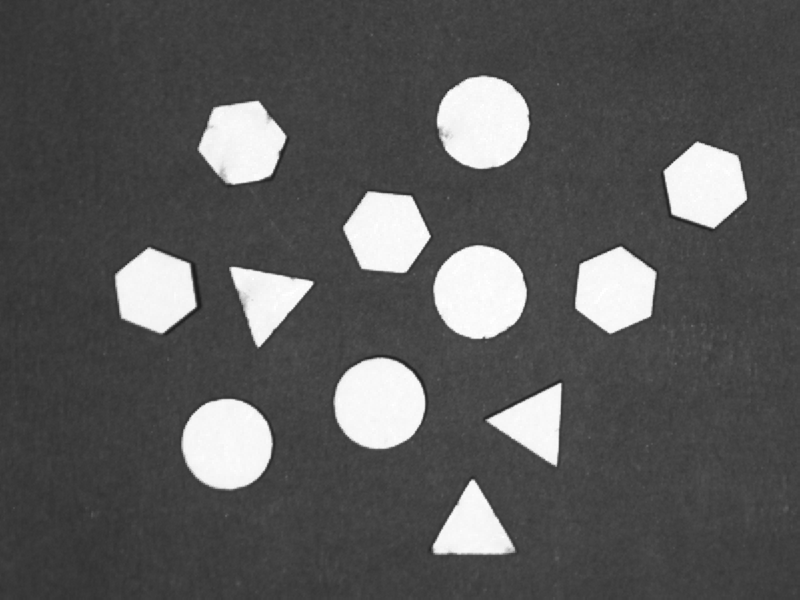
\includegraphics[width=0.4\textwidth]{./images/forms.png}
\end{center}

\Quest A partir des exemples fournis dans la section précédente (OpenCV), proposer une méthode (algorithme) à mettre en place pour détecter les éléments en fonction de leur forme. On s'intéressera notamment aux coordonnées du centre de la pièce et à leur forme.

\Manip A partir de l'exemple \textsc{camera\_flux\_lensepy\_simple.py} (en remplaçant si besoin l'image provenant de la caméra par l'ouverture d'une image fixe), mettre en oeuvre cet algorithme et tester votre code.


\noindent \rule{\linewidth}{1pt}

\textit{La suite de cette partie pourra être continuée lors de la séance 4. Vous pourrez notamment travailler par équipe de 4 pour améliorer la détection des formes et leur emplacement.}

\medskip

Pour finaliser ce mini-projet, il reste à mettre en place la détection des alignements des formes et vérifier que 3 formes du même type sont alignés...


%%%%%%%%%%%%%%%%%%%%%%%%%%%%%%%%%%%%%%%%%%%%%%%%
%%% RESSOURCES COMPLEMENTAIRES		

%\newpage
%\begin{center}
%	\begin{minipage}{2.5cm}
%	\begin{center}
%		\includegraphics[width=5cm]{../images/Logo-LEnsE.png}
%	\end{center}
%\end{minipage}\hfill
%\begin{minipage}{10cm}
%	\begin{center}
%	\textbf{Institut d'Optique Graduate School }\\[0.1cm]
%    \textbf{Interfaçage Numérique}
%
%
%	\end{center}
%\end{minipage}\hfill
%
%
%\vspace{2cm}
%
%
%{\Large \bfseries \textsc{Interfaçage Numérique}} \\[0.5cm]
%{\large \bfseries Travaux Pratiques} \\[0.2cm]
%Semestre 6
%
%\vspace{1cm}
%
%% Title
%\rule{\linewidth}{0.4mm} \\[0.4cm]
%{ \Large \bfseries\color{violet_iogs} Ressources \\[0.4cm] }
%\rule{\linewidth}{0.4mm} \\[1cm]
%{\large Bloc Vision Industrielle}
%
%\end{center}
%
%\vspace{3cm}
%
%\textbf{\large Liste des ressources}
%\begin{itemize}
%	\item ???
%\end{itemize}
%
%\vfill



%
%\includepdf[pages={1,4}, nup=1x2, pagecommand={\section{\texorpdfstring{\hspace{-1em}}{Image Processing}}}\label{doc:image_proc}]{../docs/Image_Processing.pdf}
%\includepdf[pages={5,8,12,14,16,17,18,20,21,22,23,24,25,31}, nup=1x2]{../docs/Image_Processing.pdf}

\end{document}


